%=======================================================================
%  Póster A0 vertical — Evaluación del impacto causal de los proyectos
%  de bonos de carbono sobre la deforestación en Colombia
%
%  Compilar:  pdflatex poster.tex   (dos pasadas)
%  Requiere:  beamerposter, pgfplots, booktabs, tcolorbox
%  Figuras:   figura_6_1_estudio_eventos.png, figura_6_3_cohortes.png
%=======================================================================
\documentclass[final,t]{beamer}
\usepackage[orientation=portrait,size=a0,scale=0.97]{beamerposter}
\usepackage[utf8]{inputenc}
\usepackage[T1]{fontenc}
\usepackage{helvet}
\renewcommand{\familydefault}{\sfdefault}
\usepackage{anyfontsize}
\usepackage{colortbl}
\usepackage{booktabs}
\usepackage{tabularx}
\usepackage{ragged2e}
\usepackage{amsmath}
\usepackage{graphicx}
\usepackage{tcolorbox}
\usepackage{pgfplots}
\usepackage{amssymb}
\usepackage[spanish,es-tabla]{babel}
\setlength{\aboverulesep}{0pt}
\setlength{\belowrulesep}{0pt}
\setlength{\extrarowheight}{.5ex} % para compensar el espacio visual perdido
\pgfplotsset{compat=1.18}
\tcbuselibrary{skins}

%----------------------- Paleta -----------------------
\definecolor{tinta}{HTML}{12261E}
\definecolor{dosel}{HTML}{1D4F3F}
\definecolor{papel}{HTML}{F2F4EF}
\definecolor{reduccion}{HTML}{2F7A5B}
\definecolor{brasa}{HTML}{8F3B1F}
\definecolor{amazonia}{HTML}{B8860F}
\definecolor{regla}{HTML}{C4CEC6}
\definecolor{tenue}{HTML}{5B6E63}
\definecolor{cajafondo}{HTML}{E6EBE4}
\definecolor{alertafondo}{HTML}{F4E7E0}
\definecolor{politicafondo}{HTML}{E4EFE7}
\definecolor{orofondo}{HTML}{F6ECD2}

%----------------------- Tema -------------------------
\usetheme{default}
\usecolortheme{default}
\setbeamercolor{background canvas}{bg=papel}
\setbeamercolor{normal text}{fg=tinta}
\setbeamercolor{block title}{bg=papel,fg=dosel}
\setbeamercolor{block body}{bg=papel,fg=tinta}
\setbeamerfont{block title}{series=\bfseries,size=\Large}
\setbeamertemplate{navigation symbols}{}
\setbeamertemplate{caption}[numbered]
\setbeamerfont{caption}{size=\small}
\setbeamercolor{caption name}{fg=tenue}
\setbeamercolor{itemize item}{fg=reduccion}
\setbeamertemplate{itemize item}{\raisebox{0.18ex}{\rule{0.45ex}{0.45ex}}}
\setlength{\parskip}{0.4\baselineskip}

% Título de sección con filete y referencia al capítulo de la tesis
\newcommand{\seccion}[2]{%
  \par\vspace{0.5\baselineskip}%
  {\color{dosel}\Large\bfseries #1\hfill{\color{tenue}\normalsize\mdseries #2}}\par
  \vspace{-0.35\baselineskip}%
  {\color{dosel}\rule{\linewidth}{2.2pt}}\par
  \vspace{0.25\baselineskip}%
}

% Nota de pie, cuerpo pequeño
\newcommand{\nota}[1]{{\color{tenue}\small #1\par}}

% Cifra destacada
\newcommand{\cifra}[2]{%
  \parbox[t]{0.46\linewidth}{%
    {\color{tinta}\rule{\linewidth}{2.5pt}}\\[0.25\baselineskip]
    {\color{dosel}\fontsize{50}{52}\selectfont\bfseries #1}\\[0.2\baselineskip]
    {\color{tenue}\small #2}}%
}

% Caja de contenido
\newtcolorbox{caja}[2][cajafondo]{
  colback=#1, colframe=dosel, boxrule=0pt, leftrule=5pt,
  sharp corners, left=8pt, right=8pt, top=8pt, bottom=8pt,
  title=\textbf{#2}, coltitle=tinta, fonttitle=\large,
  attach title to upper=\par\vspace{2mm}
}

\begin{document}
\begin{frame}[t]{}

%=======================================================================
%  CABECERA
%=======================================================================
\begin{tcolorbox}[colback=dosel,colframe=dosel,boxrule=0pt,sharp corners,
  left=1.2cm,right=1.2cm,top=1.0cm,bottom=1.0cm]
  {\color{papel!70}\normalsize Maestría en Economía Aplicada \quad\textbullet\quad Tesis de grado}\\[0.3cm]
  {\color{papel!40}\rule{\linewidth}{1pt}}\\[0.6cm]
  {\color{papel}\fontsize{72}{80}\selectfont\bfseries
   Evaluación del impacto causal de los proyectos de bonos de carbono
   sobre la deforestación en Colombia}\\[0.5cm]
  {\color{papel!75}\fontsize{36}{44}\selectfont\itshape
   Evidencia municipal 2001--2024 para el fortalecimiento de la política climática}\\[0.7cm]
  {\color{papel!85}\large\textbf{José David Cuervo Urrego}\quad\textbullet\quad
   \textbf{Harold Stiven Acuña Alaguna}\qquad Asesor: Jorge Luis Montero Mestre}
\end{tcolorbox}



%=======================================================================
%  FRANJA: HALLAZGO METODOLÓGICO
%=======================================================================
\begin{tcolorbox}[colback=tinta,colframe=tinta,boxrule=0pt,sharp corners,
  left=1.2cm,right=1.2cm,top=0.9cm,bottom=0.9cm]
\begin{minipage}[c]{0.36\linewidth}
  {\color{papel}\fontsize{40}{46}\selectfont\bfseries El signo del efecto depende del estimador}\\[0.6cm]
  \setlength{\leftskip}{0.9cm}\setlength{\parindent}{-0.9cm}
  \color{papel!75}\large
  \textcolor{amazonia}{\rule{0.45ex}{0.45ex}}\hspace{0.5cm}Mismo panel, mismo parámetro: TWFE positivo,
  Callaway  \& Sant'Anna negativo. \textbf{\textcolor{amazonia}{Cambio de signo, no de magnitud.}}\par\vspace{0.35cm}
  \textcolor{amazonia}{\rule{0.45ex}{0.45ex}}\hspace{0.5cm}Goodman-Bacon: \textbf{\textcolor{amazonia}{97,2\,\%}}
  del peso proviene de comparaciones limpias contra nunca tratados.\par\vspace{0.35cm}
  \textcolor{amazonia}{\rule{0.45ex}{0.45ex}}\hspace{0.5cm}El origen no son los pesos negativos, sino
  \textbf{\textcolor{amazonia}{el periodo base de comparación}} ($g-1$ frente a todo el periodo previo).\par
\end{minipage}\hfill
\begin{minipage}[c]{0.60\linewidth}
\centering
\begin{tikzpicture}[x=0.045cm,y=1cm,
   nombre/.style={anchor=east,align=right,text width=13cm,text=papel!75,font=\normalsize},
   sub/.style={anchor=east,align=right,text width=13cm,text=papel!50,font=\small},
   valor/.style={anchor=south,font=\bfseries\normalsize},
   eje/.style={anchor=north,text=papel!50,font=\normalsize}]

  % rejilla vertical
  \foreach \v in {-300,-200,-100,100,200}
    \draw[papel!22,very thin] (\v,0.95) -- (\v,-9.05);
  \draw[papel!65,dashed,semithick] (0,1.15) -- (0,-9.25);

  % --- TWFE ---
  \node[nombre] at (-400,0) {TWFE};
  \draw[brasa!80,semithick] (-105.0,0) -- (212.1,0);
  \fill[brasa!80] (0,-0.35) rectangle (53.56,0.35);
  \node[valor,text=brasa!45] at (27,0.42) {$+$53{,}56};

  % --- CS sin covariables ---
  \node[nombre] at (-400,-2) {Callaway \& Sant'Anna};
  \node[sub]    at (-400,-2.55) {sin covariables};
  \draw[reduccion!80,semithick] (-288.93,-2) -- (38.00,-2);
  \fill[reduccion!85] (-125.46,-2.35) rectangle (0,-1.65);
  \node[valor,text=reduccion!45] at (-63,-1.58) {$-$125{,}46};

  % --- CS doblemente robusta ---
  \node[nombre] at (-400,-4) {Callaway  \& Sant'Anna};
  \node[sub]    at (-400,-4.55) {doblemente robusta};
  \draw[reduccion!80,semithick] (-216.97,-4) -- (101.97,-4);
  \fill[reduccion!85] (-57.50,-4.35) rectangle (0,-3.65);
  \node[valor,text=reduccion!45] at (-29,-3.58) {$-$57{,}50};

  % --- CS muestra ponderada ---
  \node[nombre] at (-400,-6) {Callaway \& Sant'Anna};
  \node[sub]    at (-400,-6.55) {muestra ponderada *};
  \draw[reduccion!80,semithick] (-344.27,-6) -- (-12.01,-6);
  \fill[reduccion!85] (-178.14,-6.35) rectangle (0,-5.65);
  \node[valor,text=reduccion!45] at (-89,-5.58) {$-$178{,}14};

  % --- Sun-Abraham ---
  \node[nombre] at (-400,-8) {Sun  \& Abraham *};
  \draw[reduccion!80,semithick] (-239.30,-8) -- (-6.36,-8);
  \fill[reduccion!85] (-122.83,-8.35) rectangle (0,-7.65);
  \node[valor,text=reduccion!45] at (-61,-7.58) {$-$122{,}83};

  % --- escala ---
  \foreach \v/\t in {-300/$-$300,-200/$-$200,-100/$-$100,0/0,100/$+$100,200/$+$200}
    \node[eje] at (\v,-9.35) {\t};
  \node[anchor=north,text=papel!50,font=\normalsize] at (-50,-10.15)
    {ATT sobre pérdida anual de bosque (ha) \textbullet\ línea = IC 95\,\% \textbullet\ (*) intervalo que excluye el cero};
\end{tikzpicture}
\end{minipage}
\end{tcolorbox}



%=======================================================================
%  TRES COLUMNAS
%=======================================================================
\begin{columns}[t]

%-------------------- COLUMNA 1 --------------------
\begin{column}{0.305\paperwidth}
\justifying

\seccion{Problema de política}{}
\begin{itemize}
  \item El mecanismo de no causación (Ley 1819 de 2016, Decreto 926 de 2017) permite compensar
        el impuesto al carbono con créditos certificados.
  \item Ese incentivo aceleró la expansión de proyectos REDD+ sin evaluación causal previa.
  \item[\textcolor{brasa}{\rule{0.45ex}{0.45ex}}] Sobreacreditación documentada: los créditos emitidos
        equivalen a \textbf{10,7 veces} las reducciones verificables en 44 proyectos REDD+
        (Swinfield et al., 2026).
  \item Sin evidencia causal, el MADS no distingue beneficio climático real de acreditación
        no atribuible.
\end{itemize}

\vspace{0.3cm}
{\color{amazonia}\rule{3pt}{2.6cm}}\hspace{0.4cm}%
\begin{minipage}[b]{0.88\linewidth}
  {\color{dosel}\fontsize{30}{36}\selectfont\itshape
   ¿En qué medida los proyectos de bonos de carbono reducen la deforestación municipal
   en Colombia entre 2001 y 2024?}
\end{minipage}

\vspace{0.3cm}
\nota{Se evalúan tres condiciones necesarias de integridad ambiental: adicionalidad,
persistencia y desplazamiento espacial.}

\seccion{Datos}{}
\cifra{1.122}{municipios}\hfill\cifra{26.928}{observaciones municipio--año}

\vspace{0.5cm}
\cifra{88 - 99}{municipios tratados}\hfill\cifra{17 - 19}{cohortes de adopción}

\vspace{0.6cm}
\textbf{\large Resultado}
\begin{itemize}
  \item Pérdida de cobertura arbórea, Global Forest Change a 30~m (Hansen et al., 2013),
        por estadística zonal.
  \item Distribución muy asimétrica: mediana de 22~ha frente a máximos sobre 30.000~ha
        $\rightarrow$ se añade la tasa relativa al bosque base.
\end{itemize}

\textbf{\large Tratamiento}
\nota{Registros consultados y método de asignación municipal.}
\begin{center}
\begin{tabularx}{\linewidth}{Xrl}
\toprule
\rowcolor{dosel}
\textcolor{papel}{\textbf{Registro}} & \textcolor{papel}{\textbf{Proy.}} &
\textcolor{papel}{\textbf{Asignación}}\\
\midrule
Verra (API Platts/S\&P) & 101 & Punto en polígono\\
Gold Standard (API)     & 28  & Punto en polígono\\
RENARE (MADS)           & 281 & Coincidencia textual\\
Cercarbono (Excel)      & 234 & Coincidencia textual\\
OffsetsDB               & 270 & Solo descubrimiento\\
\bottomrule
\end{tabularx}
\end{center}
\nota{Se descartan ACR y CDM. Errores sistemáticos de georreferenciación corregidos por
evaluación de las cuatro combinaciones de signo e intercambio.}

\begin{caja}{Dos definiciones, no dos validaciones}
\begin{itemize}
  \item \textbf{Confianza alta:} Verra + Gold Standard, geometría exacta.
  \item \textbf{Todas las fuentes:} añade RENARE y Cercarbono, asignadas por texto.
  \item[\textcolor{amazonia}{\rule{0.45ex}{0.45ex}}] La segunda contiene a la primera:
        coincidir no es validar.
\end{itemize}
\end{caja}

\seccion{Hipótesis y contraste}{}
\begin{center}
\begin{tabularx}{\linewidth}{lX}
\toprule
\rowcolor{dosel}
\textcolor{papel}{\textbf{Hipótesis}} & \textcolor{papel}{\textbf{Veredicto empírico}}\\
\midrule
H1. ATT negativo          & Signo consistente, sin significancia agregada\\
H2. Sin dinámicas previas & Pretendencias sin divergencia creciente\\
H3. Efecto persistente    & Sin reversión, sin precisión para afirmarlo\\
H4. Fuga hacia vecinos    & No detectable\\
H5. Efecto heterogéneo    & Solo la dimensión regional se sostiene\\
\bottomrule
\end{tabularx}
\end{center}

\end{column}

%-------------------- COLUMNA 2 --------------------
\begin{column}{0.305\paperwidth}
\justifying

\seccion{Estrategia empírica}{}
\nota{Diferencias en diferencias con adopción escalonada. Parámetro de interés, identificado
contra el periodo previo a la adopción:}
\begin{tcolorbox}[colback=cajafondo,colframe=regla,boxrule=0.8pt,sharp corners]
\centering
\[
  ATT(g,t) \;=\; \mathbb{E}\!\left[Y_{t}-Y_{g-1}\,\middle|\,G_{g}=1\right]
               \;-\; \mathbb{E}\!\left[Y_{t}-Y_{g-1}\,\middle|\,C=1\right]
\]
\raggedright\nota{$G_g$: cohorte que adopta en el año $g$. $C$: municipios aún no tratados.
La agregación dinámica produce el estudio de eventos; la simple, el ATT global.}
\end{tcolorbox}

\nota{Especificación de contraste metodológico:}
\begin{tcolorbox}[colback=cajafondo,colframe=regla,boxrule=0.8pt,sharp corners]
\centering
\[
  Y_{it} \;=\; \alpha_i + \delta_t + \beta D_{it} + \varepsilon_{it}
\]
\end{tcolorbox}

\begin{itemize}
  \item Emparejamiento completo por puntaje de propensión sobre doce covariables
        de línea base: clima, accesibilidad, conflicto y bosque base.
  \item Control efectivo de 156,5 municipios frente a 82 con emparejamiento uno a uno;
        87 de 88 tratados conservan pareja.
  \item Robustez: Sun y Abraham (2021), imputación de Borusyak et al. (2024),
        sensibilidad de Rambachan y Roth (2023).
\end{itemize}

\seccion{Efecto promedio}{}
\nota{Tabla 6.1. ATT sobre la pérdida de bosque. (*) intervalo que excluye el cero al 5\,\%.}
\begin{center}
\begin{tabularx}{\linewidth}{Xrr}
\toprule
\rowcolor{dosel}
\textcolor{papel}{\textbf{Especificación}} & \textcolor{papel}{\textbf{ATT (ha)}} &
\textcolor{papel}{\textbf{EE}}\\
\midrule
Alta · sin covariables      & \textcolor{reduccion}{\textbf{$-$125,46}} & 83,40\\
Alta · doblemente robusta   & \textcolor{reduccion}{\textbf{$-$57,50}}  & 81,36\\
Alta · muestra ponderada *  & \textcolor{reduccion}{\textbf{$-$178,14}} & 84,76\\
Todas · sin covariables     & \textcolor{reduccion}{\textbf{$-$105,86}} & 70,63\\
Todas · doblemente robusta  & \textcolor{reduccion}{\textbf{$-$54,86}}  & 72,06\\
Todas · muestra ponderada * & \textcolor{reduccion}{\textbf{$-$149,70}} & 70,15\\
\bottomrule
\end{tabularx}
\end{center}
\begin{itemize}
  \item Las seis coinciden en signo negativo.
  \item[\textcolor{brasa}{\rule{0.45ex}{0.45ex}}] Las dos significativas son las que
        \textbf{no} ajustan el desbalance residual en bosque base y distancia al mercado.
  \item La magnitud varía por un factor cercano a tres entre especificaciones.
\end{itemize}

\seccion{Tendencias paralelas y persistencia}{}
\begin{center}
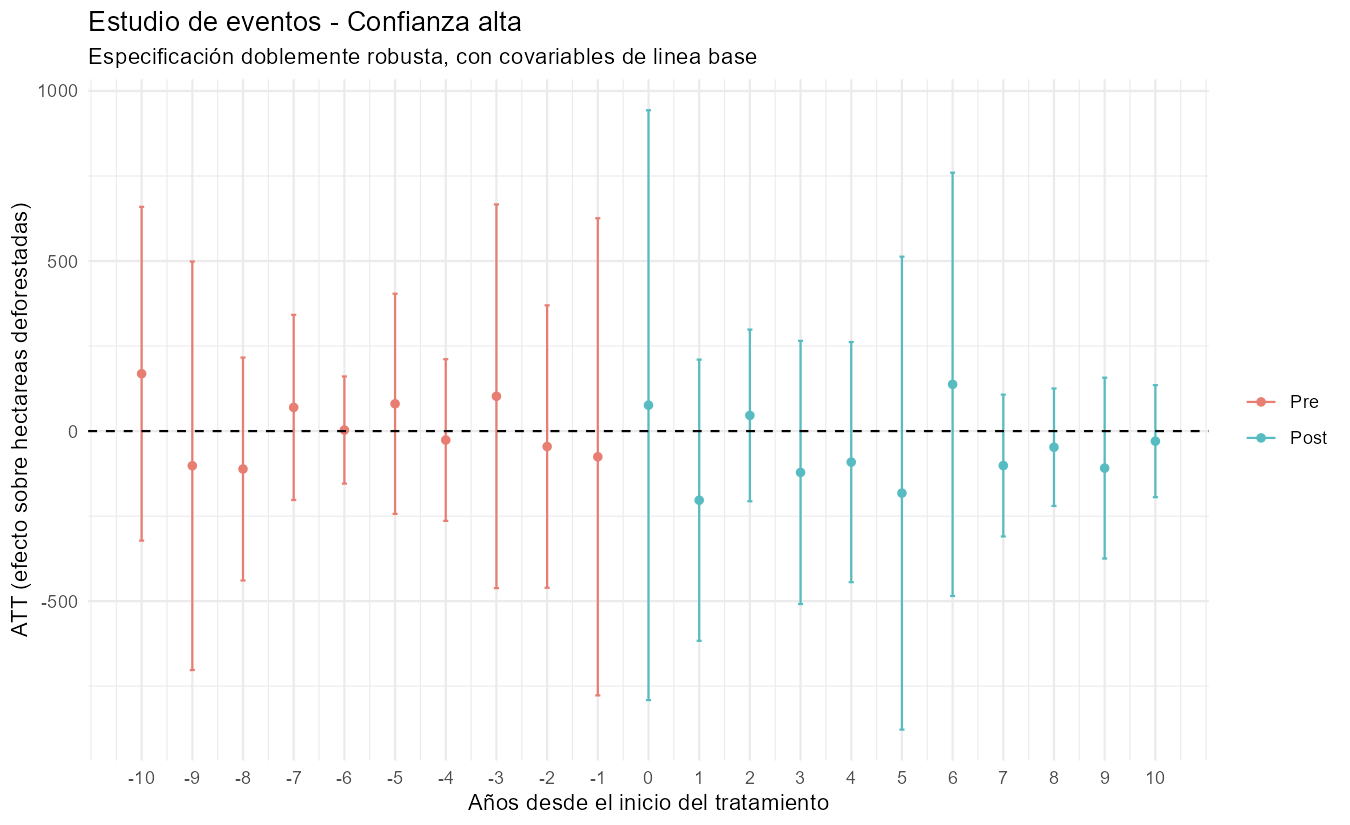
\includegraphics[width=0.96\linewidth]{figura_6_1_estudio_eventos.png}
\end{center}
\nota{Figura 6.1. Estudio de eventos, confianza alta, especificación doblemente robusta.}
\begin{itemize}
  \item Coeficientes pretratamiento en torno a cero, sin divergencia creciente.
  \item Postratamiento mayoritariamente negativos, ninguno individualmente significativo.
  \item[\textcolor{amazonia}{\rule{0.45ex}{0.45ex}}] Sin reversión sistemática, pero tampoco
        evidencia de persistencia. \textcolor{amazonia}{\textbf{[\textbullet\ prueba conjunta y
        $\bar{M}$ mínimo]}}
\end{itemize}

\seccion{Heterogeneidad por cohorte}{}
\begin{center}
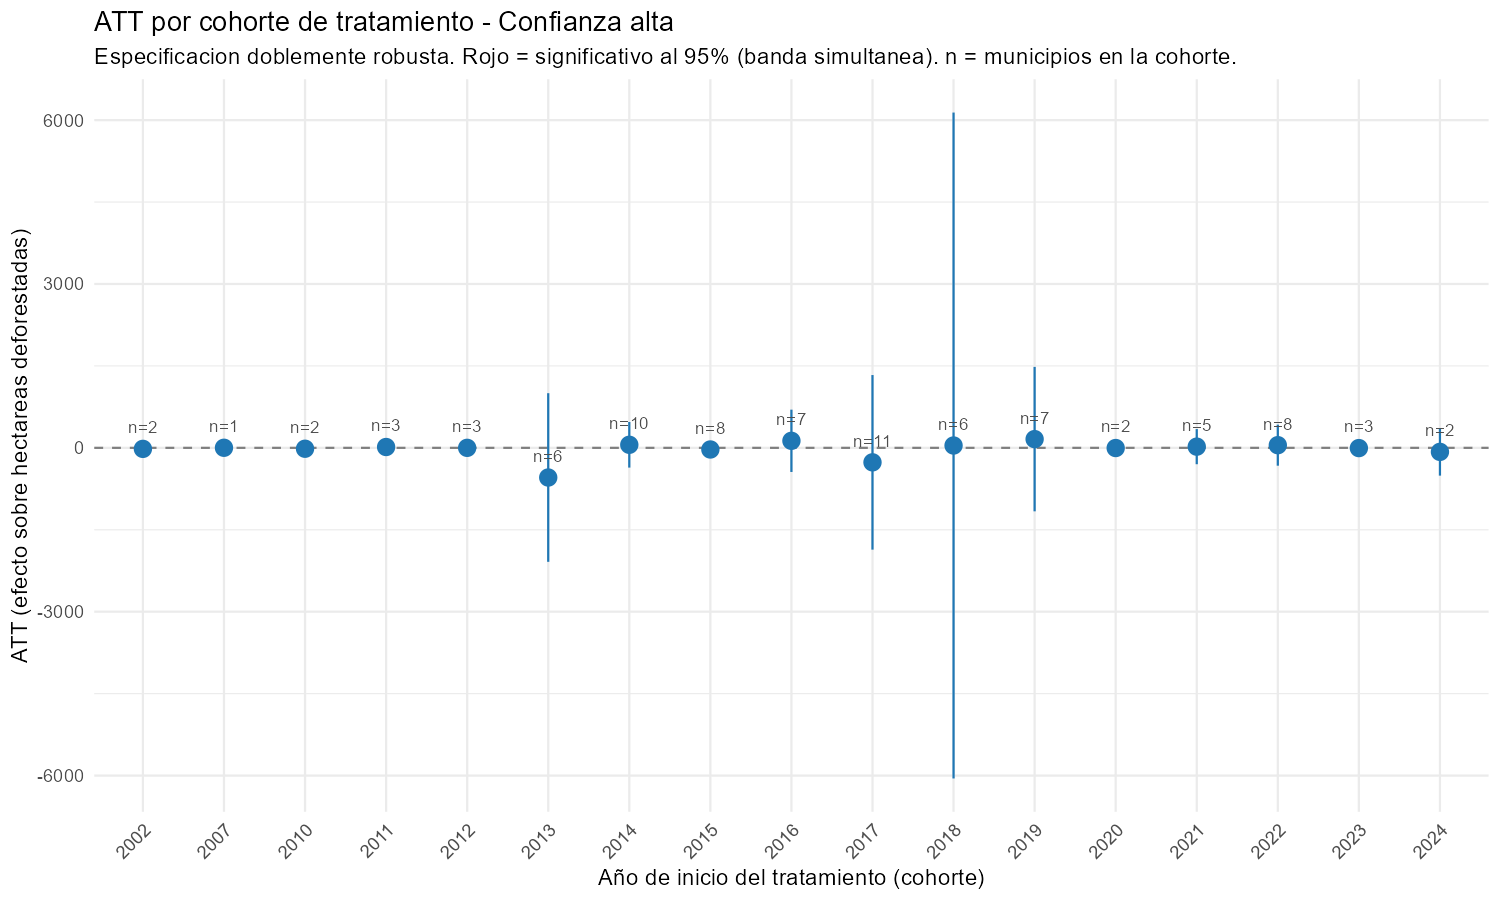
\includegraphics[width=0.92\linewidth]{figura_6_3_cohortes.png}
\end{center}
\nota{Figura 6.3. ATT por cohorte de adopción, confianza alta. $n$ = municipios por cohorte.}
\nota{Cohortes de uno a doce municipios: los signos opuestos se compensan en el promedio y la
dispersión no separa heterogeneidad genuina de ruido muestral.}

\end{column}

%-------------------- COLUMNA 3 --------------------
\begin{column}{0.305\paperwidth}
\justifying

\seccion{Heterogeneidad territorial}{}
\nota{Tabla 6.5. ATT por región. (*) significativo al 5\,\%.}
\begin{center}
\begin{tabularx}{\linewidth}{Xrrr}
\toprule
\rowcolor{dosel}
\textcolor{papel}{\textbf{Región}} & \textcolor{papel}{\textbf{ha (alta)}} &
\textcolor{papel}{\textbf{tasa (alta)}} & \textcolor{papel}{\textbf{tasa (todas)}}\\
\midrule
Andina    & $+$3,06    & $-$0,024\,\%   & $+$0,009\,\%\\
Caribe    & \textcolor{brasa}{\textbf{$+$38,66}} & $+$0,097\,\% & $+$0,205\,\%\\
Pacífica  & \textcolor{reduccion}{\textbf{$-$63,32}} & $+$0,054\,\% & $+$0,068\,\%\\
Orinoquía & \textcolor{reduccion}{\textbf{$-$223,14}} & $-$0,060\,\% & $-$0,060\,\%\\
\rowcolor{orofondo}
\textbf{Amazonía} & \textbf{$-$1.297,41} & \textbf{$-$0,177\,\% *} & \textbf{$-$0,163\,\% *}\\
\bottomrule
\end{tabularx}
\end{center}
\begin{itemize}
  \item[\textcolor{amazonia}{\rule{0.45ex}{0.45ex}}] Amazonía: único resultado significativo
        bajo ambas definiciones, y solo en tasa.
  \item Andina: 45 municipios tratados y el menor error estándar. Es el
        \textbf{nulo mejor estimado} del análisis.
\end{itemize}

\begin{caja}[alertafondo]{La magnitud amazónica exige cautela}
\begin{itemize}
  \item El ATT en tasa equivale a $\sim$80\,\% de la tasa media posterior: reducción implícita
        del orden de 44\,\%.
  \item Difícil de conciliar si los proyectos cubren una fracción minoritaria del bosque municipal.
  \item La tabla reúne veinte contrastes por subgrupo.
        \textcolor{amazonia}{\textbf{[\textbullet\ $p$-valores Holm y cobertura mediana]}}
\end{itemize}
\end{caja}

\seccion{Desplazamiento espacial}{}
\nota{Vecindad tipo reina; muestra restringida a municipios nunca tratados directamente.}
\begin{center}
\begin{tabularx}{\linewidth}{Xrr}
\toprule
\rowcolor{dosel}
\textcolor{papel}{\textbf{Enfoque}} & \textcolor{papel}{\textbf{Coef. (ha)}} &
\textcolor{papel}{\textbf{IC 95\,\%}}\\
\midrule
Callaway  \& Sant'Anna       & $+$41,23 & [$-$93,8 ; 176,2]\\
TWFE con rezago espacial  & \textcolor{brasa}{\textbf{$+$279,18}} & [74,7 ; 483,7]\\
\bottomrule
\end{tabularx}
\end{center}
\begin{itemize}
  \item No es coherente descartar TWFE para el efecto directo y apoyarse en él para afirmar fuga.
  \item Sin evidencia detectable de desplazamiento; tampoco potencia para descartarlo.
\end{itemize}

\seccion{Limitaciones}{}
\begin{itemize}
  \item[\textcolor{brasa}{\rule{0.45ex}{0.45ex}}] El hallazgo amazónico admite una explicación
        alternativa: el aumento de deforestación tras la salida de las FARC-EP desde 2016.
  \item[\textcolor{brasa}{\rule{0.45ex}{0.45ex}}] El resultado mide pérdida de cobertura arbórea,
        no conversión de bosque natural: limita la comparabilidad con el IDEAM.
  \item[\textcolor{brasa}{\rule{0.45ex}{0.45ex}}] Excluir vecinos del control rompe el soporte
        común: limitación estructural del diseño, no falla de robustez.
  \item[\textcolor{brasa}{\rule{0.45ex}{0.45ex}}] La identificación contra un año base único es
        sensible a la volatilidad interanual.
  \item[\textcolor{brasa}{\rule{0.45ex}{0.45ex}}] Cobertura de registros incompleta y margen de
        error en la asignación textual.
\end{itemize}

\seccion{Implicaciones para el MADS}{}
\begin{caja}[politicafondo]{}
\begin{itemize}
  \item \textbf{Gestión regulatoria.} La ausencia de efecto agregado no respalda una acreditación
        uniforme: se requieren criterios diferenciados por contexto territorial.
  \item \textbf{Sistema MRV.} RENARE no expone coordenadas ni municipio estructurado;
        la georreferenciación obligatoria es condición previa para evaluar.
  \item \textbf{Priorización.} El único efecto significativo se concentra en la Amazonía,
        donde coinciden bosque primario y presión de frontera.
\end{itemize}
\end{caja}

\end{column}
\end{columns}

\vfill

%=======================================================================
%  PIE
%=======================================================================
\colorbox{tinta}{%
\begin{minipage}[t]{\dimexpr\paperwidth-2.4cm\relax}
\vspace{0.7cm}
\hspace{0.8cm}%
\begin{minipage}[t]{0.63\linewidth}
  {\color{papel!65}\small\textbf{\color{papel}Referencias principales.}
  Callaway y Sant'Anna (2021) \textbullet\ Sun y Abraham (2021) \textbullet\ Goodman-Bacon (2021)
  \textbullet\ De Chaisemartin y D'Haultf\oe uille (2020) \textbullet\ Borusyak et al. (2024)
  \textbullet\ Rambachan y Roth (2023) \textbullet\ Hansen et al. (2013)
  \textbullet\ Guizar-Coutiño et al. (2022) \textbullet\ Swinfield et al. (2026)
  \textbullet\ Probst et al. (2024) \textbullet\ Blanton et al. (2024).}
\end{minipage}\hfill
\begin{minipage}[t]{0.32\linewidth}
  {\color{papel!65}\small\textbf{\color{papel}Reproducibilidad.}
  Panel en Python (pandas, GeoPandas, Google Earth Engine); estimación en R
  (\textit{did}, \textit{MatchIt}, \textit{spdep}). Los campos
  \textcolor{amazonia}{\textbf{[\textbullet]}} están en verificación.}
\end{minipage}
\hspace{0.8cm}
\vspace{0.7cm}
\end{minipage}}

\end{frame}
\end{document}
